\section{Data engine}

\begin{figure}[!t]
\centering
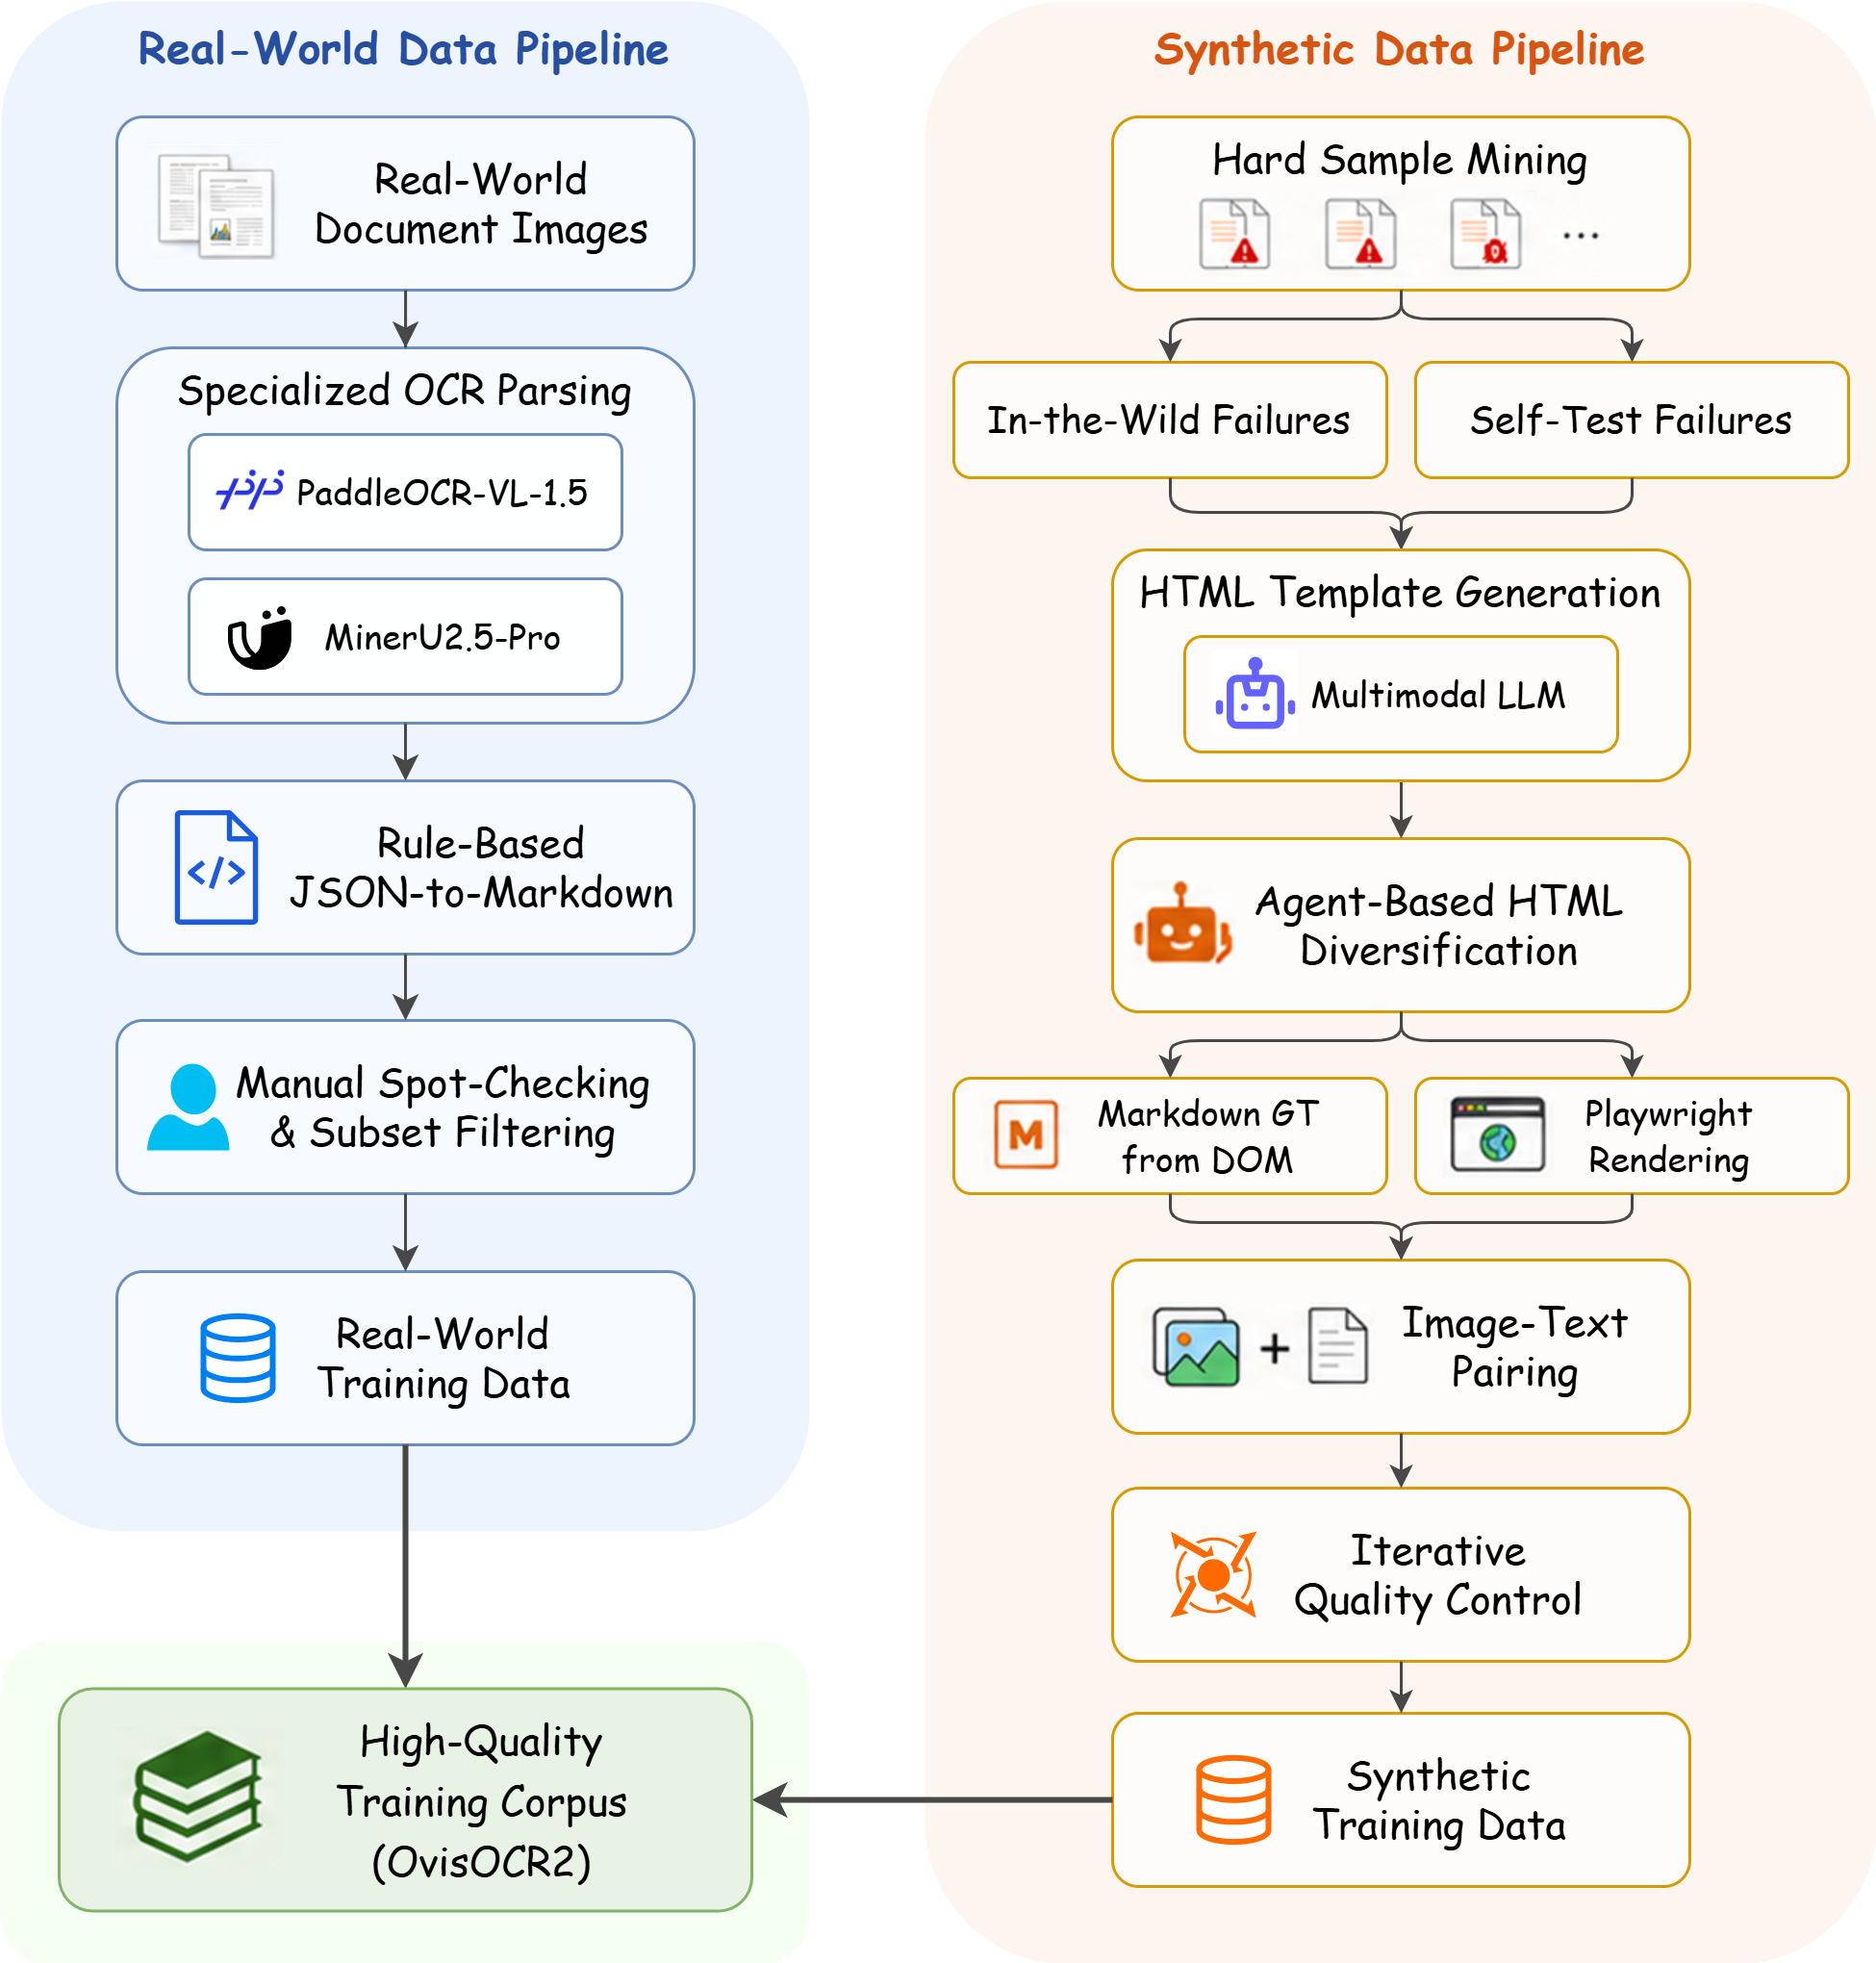
\includegraphics[width=0.88\linewidth]{figures/data_pipeline.png}
\caption{Architecture of the data engine}
\label{fig:data_pipeline}
\end{figure}

Training an end-to-end document parser requires supervision that is accurate at multiple levels: fine-grained text transcription, structurally valid serialization, faithful recovery of tables and formulas, and globally coherent reading order. These requirements make data preparation itself a key part of the system design. No single data source is sufficient: real-world documents provide natural layouts and varied visual conditions, but their annotations are noisy and difficult to standardize; synthetic documents offer controllable training targets and scalable coverage, but may suffer from limited realism if synthesized naively. To address this, we build a data engine composed of two complementary pipelines, a real-world data pipeline and a synthetic data pipeline, as shown in Fig.~\ref{fig:data_pipeline}.

\begin{itemize}
    \item \textbf{Real-world data pipeline.}
    This pipeline transforms large-scale real-world document images into reliable document-to-Markdown training data. It exposes the model to real-world visual distributions, including diverse templates, scan qualities, font styles, languages, layout structures, tables, formulas, figures, and other heterogeneous document elements.

    \item \textbf{Synthetic data pipeline.}
    This pipeline complements real-world data by synthesizing controllable document samples with precise ground-truth annotations. Its role is to expand the long-tail coverage of the training distribution, especially for rare or difficult cases that are underrepresented in naturally collected documents, such as table topologies, dense formula-text interleaving, extreme multi-column layouts, and long Markdown outputs.
\end{itemize}

\subsection{Real-world data pipeline}

The real-world pipeline turns document images into training data through conversion and filtering. It first obtains structured outputs from OCR parsers, normalizes them into a common Markdown schema, and then filters the resulting Markdown outputs through rule-based checks and subset-level spot-checking. In this process, parser outputs are used as structured candidates rather than final labels; deterministic conversion and conservative filtering are applied before the data enter the training corpus to improve serialization consistency and structural validity.

\subsubsection{Rule-based structured parsing and Markdown serialization}

For each document image, the real-world data pipeline uses a specialized OCR parser, either PaddleOCR-VL-1.5~\cite{paddleocrvl15} or MinerU2.5-Pro~\cite{mineru25pro}, to obtain structured parsing results. Instead of directly using the raw Markdown strings produced by these systems, we parse their structured JSON responses and convert them into a unified Markdown format through source-specific rules. Each parser output is treated as an ordered list of blocks, where each block contains its category, recognized content, bounding box, and optional parser-specific metadata. The data engine then applies a JSON-to-Markdown converter to normalize these heterogeneous block structures.

The conversion rules are designed around the following principles:

\begin{itemize}
    \item \textbf{Strict category validation.}
    The converter accepts only predefined document categories. MinerU2.5-Pro categories are grouped into text-like elements, tables, visual elements such as images and charts, and container-like blocks that do not directly contribute Markdown content. PaddleOCR-VL-1.5 uses a broader layout vocabulary, covering titles, paragraphs, formulas, tables, figures, headers, footers, seals, footnotes, vertical text, and other document regions. Unknown or unsupported categories are rejected rather than silently ignored, reducing the risk of corrupted annotations entering the training set.

    \item \textbf{Text-block normalization.}
    Text-like blocks with empty content or unreadable placeholders are skipped and recorded by a filtering flag. For MinerU2.5-Pro, adjacent text blocks marked with \texttt{merge\_prev} are merged conservatively: a block is merged only when a valid previous text block exists and the current content is non-empty. Chinese text is concatenated directly, while non-Chinese text is separated with a space. For title blocks, the converter further derives Markdown heading levels from numbering patterns such as decimal section indices, Roman numerals, alphabetic markers, and Chinese section markers, while avoiding over-promotion of year-like numeric titles.

    \item \textbf{Formula normalization.}
    Mathematical expressions are normalized into a unified LaTeX-style Markdown representation. For MinerU2.5-Pro, inline wrappers such as \texttt{\textbackslash(...\textbackslash)} are converted into \texttt{\$...\$}, and display wrappers such as \texttt{\textbackslash[...\textbackslash]} are converted into \texttt{\$\$...\$\$}. Redundant spaces inside math delimiters are removed, line breaks within math wrappers are collapsed, and escaped dollar signs are protected during conversion. Code blocks and inline code spans are excluded from formula rewriting. For PaddleOCR-VL-1.5, the converter applies lightweight post-processing to trim spaces inside single-dollar inline formulas after block concatenation.

    \item \textbf{Table normalization.}
    Table blocks are required to contain valid HTML table structures. Empty tables, non-table contents, malformed table outputs, or repeated tail fragments are filtered out. MinerU2.5-Pro tables are normalized by adding \texttt{border=1} to the \texttt{<table>} tag when the border attribute is absent. PaddleOCR-VL-1.5 tables are sanitized by removing unnecessary HTML style attributes.

    \item \textbf{Visual-region normalization.}
    Visual regions such as figures, charts, header images, and footer images are represented as HTML image tags rather than textual descriptions. Their bounding boxes are normalized to the range $[0,1000)$ and serialized as \\ \texttt{<img src="images/bbox\_left\_top\_right\_bottom.jpg" />}.

    \item \textbf{Parser-specific high-risk cases.}
    Some categories require additional validation. For example, PaddleOCR-VL-1.5 seal and figure-title regions may be wrapped in HTML-like containers; the converter extracts clean text from these containers and rejects empty results. Seal blocks are further checked against layout confidence to remove unreliable detections.
\end{itemize}

After block-level normalization, all valid block contents are concatenated in parser-provided block order using double newlines. The converter also applies pre-filtering checks to remove samples with no valid text-bearing content, duplicated source images, obvious trailing repetitions, or other severe parser-side failures. The resulting Markdown is still not treated as final training data. Rule-based normalization and pre-filtering can remove obvious format and parser failures, but they cannot fully verify whether the content matches the source image. Therefore, we further introduce a spot-checking stage to assess content correspondence and global consistency before retaining the sample for training.

\subsubsection{Manual spot-checking and subset filtering}

We organize candidate datasets according to the data source, parser type, document domain, and conversion configuration. For each dataset subset, we randomly sample document--Markdown pairs and manually compare the converted Markdown with the original document images. The inspection checks whether the serialized Markdown matches the source image along the following dimensions:
\begin{itemize}
    \item \textbf{Text correspondence.}
    We check whether the Markdown output preserves the textual content in the image, without missing text, inserted text, or recognition errors.

    \item \textbf{Formula accuracy.}
    We render formulas according to LaTeX syntax and check whether the rendered results match the formulas in the image.

    \item \textbf{Table alignment.}
    We inspect whether table rows, columns, headers, and cell contents correspond to the original table, especially for dense tables and merged cells.

    \item \textbf{Visual-region alignment.}
    We render the bounding boxes encoded in HTML image tags on the original document image and check whether they cover the intended figures or charts.

    \item \textbf{Reading-order consistency.}
    We examine whether the sampled outputs follow natural human reading order, especially in multi-column pages and pages with dense mixtures of text, formulas, tables, and visual regions.
\end{itemize}

This stage is intentionally conservative. The goal is not to rewrite or repair the converted annotations through free-form generation, but to prevent low-quality data subsets from degrading the training corpus. When a subset contains only occasional minor errors, we retain it together with the sample-level filters applied during rule-based conversion. In contrast, when a subset exhibits frequent errors, it is removed from the training corpus.

\subsection{Synthetic data pipeline}

The synthetic data pipeline follows a source-of-truth principle, generating both the document image and its Markdown target from the same HTML source instead of deriving the target by parsing the rendered image. This design makes the training targets deterministic and avoids parser-derived noise in synthetic labels. The pipeline starts by mining hard samples identified through multi-faceted assessments, uses a multimodal model to convert mined hard samples into initial HTML templates, employs an agent-based generation procedure to expand them into diverse HTML pages, derives Markdown ground truth from the structured source, renders document images with Playwright~\cite{playwright}, and finally packages the resulting image-text pairs into training data after quality inspection.

\subsubsection{Hard sample mining for HTML template generation}

The synthetic data pipeline begins with hard sample mining. Instead of randomly synthesizing generic document pages, we first collect difficult samples from failure cases identified through multi-faceted assessments. These samples are selected when they reveal underrepresented document patterns, such as table-heavy layouts, irregular document structures, header/footer interference, handwritten regions, page-number ambiguity, and complex reading-order patterns.

Each mined hard sample is treated not merely as an isolated failure, but as evidence of a reusable synthesis pattern. We analyze the visual and structural factors behind the failure and group samples with similar typography, table structure, page organization, and localization requirements into the same synthesis family. This grouping allows one template to cover a class of related failure modes rather than overfitting to a single page.

Given a representative hard sample or a cluster of similar hard samples, we use a multimodal model to infer the visual and structural intent of the document. The model converts the observed hard sample into an initial HTML template that preserves the key layout structure needed for subsequent diversification. For elements requiring accurate localization, the template uses explicit DOM spans or element-level wrappers, enabling tight bounding boxes to be recovered during rendering.

The generated HTML template is therefore not a final synthetic sample, but a programmatic abstraction of the mined hard sample distribution. It preserves the challenging factors observed in real failures while exposing controllable variables for subsequent diversification. This hard-sample-centric design converts observed errors into scalable document generators with clean training targets.

\subsubsection{Agent-based HTML diversification}

After obtaining the initial template, we use an agent-based generation procedure to expand the template into a diverse set of HTML pages. The agent edits and extends the HTML template while preserving the visual identity and structural intent of the seed template. This procedure supports iterative code refinement, validity checking, and controlled diversification.

The diversification process introduces randomness at both content and structure levels. Content-level variation covers semantic fields, textual length, numerical values, formulas, and domain-specific terminology. Structure-level variation covers table structure, section hierarchy, page organization, and visual-region placement. Together, these variations expand each seed template into a synthesis family with diverse content and layout configurations.

To keep labels valid during diversification, the agent is constrained by validity rules. Each generated page must remain renderable, visually plausible, category-compliant, and convertible into valid Markdown. The pipeline further maintains domain-specific randomized content pools, allowing synthetic content to vary semantically while keeping the generated labels clean and consistent. This ensures that the synthetic data are large in scale, structurally diverse, and reliably annotated.

\subsubsection{Markdown ground truth generation}

For each diversified HTML page, the data engine generates the Markdown ground truth directly from the corresponding HTML source. The serializer maps source elements into the target Markdown format while preserving their intended structure and reading order, with separate rules for each element type:
\begin{itemize}
    \item \textbf{Text elements.}
    Text nodes, paragraphs, section titles, list items, headers, footers, and footnotes are serialized as standard Markdown text.

    \item \textbf{Tables.}
    Table elements are represented as HTML snippets \texttt{<table>...</table>}, so that both cell content and table structure are retained.

    \item \textbf{Formulas.}
    Mathematical expressions are serialized in LaTeX-style Markdown. Inline formulas and display formulas are represented with consistent math delimiters so that the target format remains compatible with the training format.

    \item \textbf{Visual regions.}
    Each visual region is serialized as an HTML image tag. The coordinates are obtained from the rendered DOM, scaled to $[0,1000)$, and written as \\ \texttt{<img src="images/bbox\_left\_top\_right\_bottom.jpg" />}.
\end{itemize}

Reading order is assigned at the page level. The serializer uses document-type-aware rules rather than a single global spatial heuristic. For regular single-column pages, elements are ordered primarily from top to bottom and secondarily from left to right. For multi-column layouts, the page is partitioned into column regions according to the template layout or the normalized bounding boxes; elements within each column are serialized from top to bottom, and columns are traversed from left to right. For structured elements such as tables, lists, formulas, and anchored visual regions, the serializer preserves their internal DOM order and template-defined associations.

\subsubsection{Document image rendering}

In parallel with Markdown generation, the same HTML page is rendered into a document image. We use Playwright~\cite{playwright} for browser-based rendering, which preserves realistic typography, spacing, table strokes, color styles, wrapping behavior, and page-level layout details. The viewport is automatically adjusted to fit the document canvas, and page boundary handling is applied when necessary to avoid invalid crops, incomplete bottom regions, or mask artifacts.

During rendering, the data engine records element-level geometry from the DOM for elements that require bounding boxes. Explicit spans and element wrappers allow the pipeline to obtain tight bounding boxes for text or visual elements. These boxes are normalized to the target coordinate range and remain consistent with the final screenshot. When visual augmentation is applied, such as mild rotation or other geometric perturbations, the corresponding coordinate transformations are applied to the labels as well.

\subsubsection{Iterative quality control}

Before large-scale generation, we perform a preview-and-iteration procedure. A small batch of samples is first rendered for visual inspection. The inspection focuses on whether the synthesized pages match the intended hard sample style in typography, table layout, page organization, visual-region localization, and reading-order details. If layout defects are observed, the HTML template, agent diversification rules, or rendering parameters are revised before scaling.

After the preview passes inspection, the pipeline expands the randomized content pools and generates samples at scale. The large-scale generation stage supports multi-threaded rendering and writes paired images and labels together with augmented variants when applicable.

The quality control stage removes samples with rendering or pairing failures, empty or degenerate Markdown targets, structural errors, localization errors, or duplicated outputs. Final dataset size is verified across image files, label files, augmented variants, and metadata records before the samples are admitted into the training dataset.

Through this pipeline, we obtain synthetic Markdown training data that are both controllable and precise. The synthetic data pipeline complements the real-world data pipeline by expanding long-tail coverage while preserving clean ground truth and faithful image-text alignment.
